
\subsection{W\_EMAP, Version Windows based map program} 

Program and documentation by \textbf{Fernando Carrilho}, fernando.carrilho@meteo.ptu\newline
Program must be installed in addition to SEISAN.

\index{Fault plane solution, plot}\index{Plotting epicenters} 
This program was developed to be used on seismic routine processing. Its main features are the capability of allowing visualization of epicentre locations, seismic stations, error ellipses, coastlines, macroseismic data, focal mechanisms (one or many) and simplified tectonics. From the previous public version (4.1), some bugs were corrected and new features added. In particular:  cartographic deformation is taken into account in error ellipses and station-epicentral path draws; some bugs on printing were corrected; compacted seisan files can be used within `additional events' representation; travel time curves can now be displayed; simplified relief can be displayed (if available as a MAP file); more than one file can be used for each category layer (coastlines, tectonic, relief and places names). 

The program can be integrated within the SEISAN environment, since it uses SEISAN parameter files, macrosseismic files, MAP files and station/model files. 

\begin{figure}
\htmlimage{scale=2.0}
\centerline{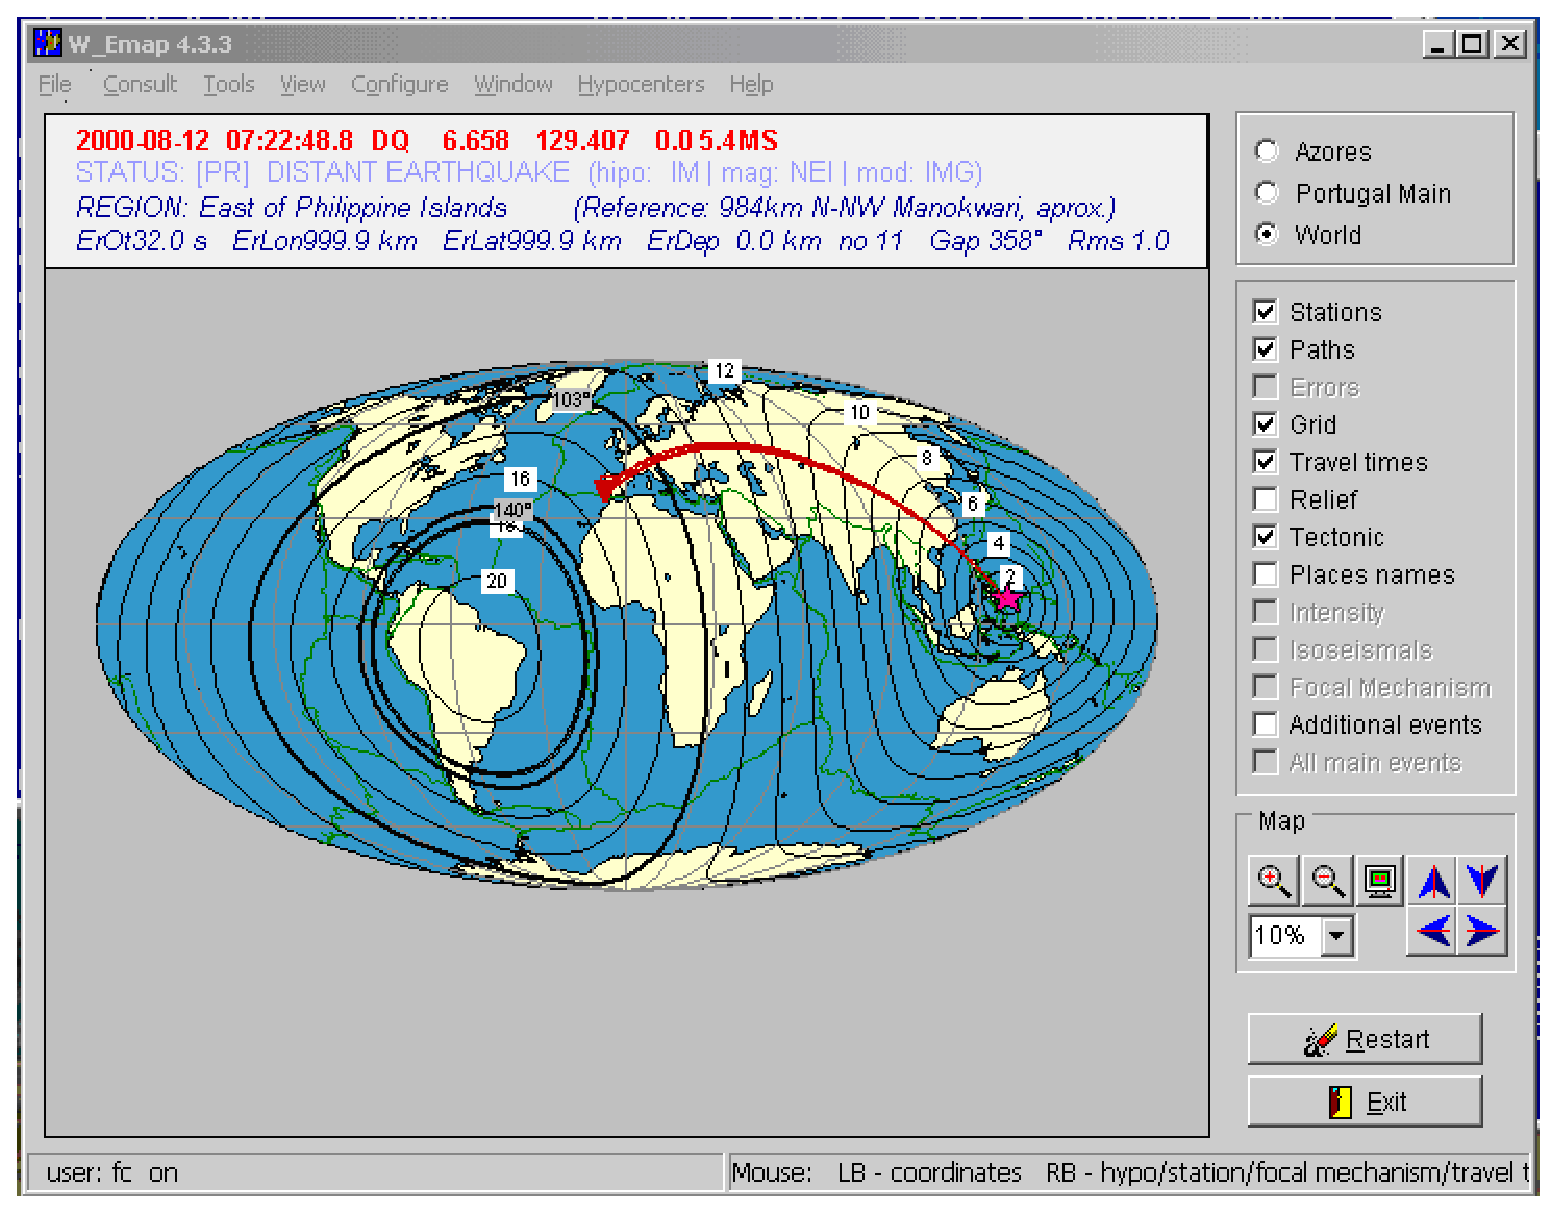
\includegraphics[width=0.9\linewidth]{fig/fig31}}
\caption{Example for plot using w\_emap (example not latest version).}
%\label{fig:}
\end{figure}


If the program is called from EEV or from the command line as W\_EMAP, then it displays information contained in \texttt{hyp.out} file, generated by the HYPOCENT \citep{lienert1994} location program, included in SEISAN, in the settable working directory. \newline
During the first run, user is driven to edit the configuration file w\_emap.def that is created in the users personal directory (SEISAN\_TOP/DAT/users/<username>), where most of the program parameters can be changed. \newline
The program can automatically detect changes in the \texttt{hyp.out} file so the user 
\underline{doesn't need to restart} the program each time the epicentre changes. \newline
The program can also display epicentres contained in any SEISAN parameter file, where the user may choose between one single epicentre and all epicentres at the same time. Double clicking the right mouse button will change the active epicentre to the one picked. 

Multi-user individual configurations (color schemes, additional event files, tectonic files, coastline files, relief files, cartographic projections, etc.) are supported. 
The program also has an option for Google Earth and Google map.. \index{Google Earth} Installation 
All the files are included in the distribution file w\_emap.exe. To install it, you just execute this install script and make sure W\_EMAP is installed under \_SEISMO\_TOP (Usually \\seismo). 
The manual will only be found in INF after installation. The current version of W\_EMAP is 4.8.2 but the manual has not been updated since version 4.6. 
An important new option is be able to directly plot a file with many hypocenters with the command w�emap filename. 
Known problem: Thre must be a type 7 line in S-file in order to be 
able to plot a focal mechanism. Some versions of w\_emap plot some 
of the fault plane solutions with inverted colors. \index{W\_EMAP} 

